\documentclass[11pt,letterpaper]{article}
\usepackage[T1]{fontenc}
\usepackage{lmodern}
\usepackage[margin=1in]{geometry}
\usepackage{amsmath,amssymb,amsthm,mathtools}
\usepackage{microtype,booktabs,tabularx,array,enumitem}
\usepackage{xcolor,graphicx,fancyhdr}
\usepackage[most]{tcolorbox}
\usepackage{hyperref}
\hypersetup{colorlinks=true,linkcolor=blue!45!black,citecolor=blue!45!black,
urlcolor=blue!45!black,pdftitle={Sharp Gaussian Quadratic Concentration from Signed Spectral Moments},
pdfauthor={ChatGPT}}
\definecolor{ink}{HTML}{173D52}
\definecolor{accent}{HTML}{126782}
\definecolor{pale}{HTML}{F0F6F8}
\pagestyle{fancy}\fancyhf{}
\fancyhead[L]{\small\textcolor{ink}{Gaussian quadratic concentration}}
\fancyhead[R]{\small Signed spectral moments}
\fancyfoot[C]{\thepage}
\setlength{\headheight}{14pt}
\setlength{\emergencystretch}{2em}
\setlist{itemsep=3pt,topsep=5pt}
\numberwithin{equation}{section}
\newtheorem{theorem}{Theorem}[section]
\newtheorem{proposition}[theorem]{Proposition}
\newtheorem{lemma}[theorem]{Lemma}
\newtheorem{corollary}[theorem]{Corollary}
\theoremstyle{definition}\newtheorem{definition}[theorem]{Definition}
\theoremstyle{remark}\newtheorem{remark}[theorem]{Remark}
\newcommand{\E}{\mathbb E}
\newcommand{\PP}{\mathbb P}
\newcommand{\R}{\mathbb R}
\newcommand{\tr}{\operatorname{tr}}
\newcommand{\diag}{\operatorname{diag}}
\newcommand{\op}{\mathrm{op}}
\newcommand{\Var}{\operatorname{Var}}
\newcommand{\supp}{\operatorname{supp}}
\newcommand{\dd}{\,\mathrm d}
\newcommand{\cstar}{c_{\mathrm{univ}}}
\newcommand{\scrit}{s_{\mathrm{crit}}}
\newcommand{\cRad}{C_{\mathrm R}}
\newcommand{\jRad}{J_{\mathrm R}}
\newcommand{\bRad}{B_{\mathrm R}}

\begin{document}
\begin{titlepage}
\vspace*{0.6in}
{\color{accent}\sffamily\large RESEARCH MANUSCRIPT\par}
\vspace{0.3in}
{\color{ink}\LARGE\bfseries Sharp Gaussian Quadratic Concentration\par}
\vspace{0.08in}
{\color{ink}\LARGE\bfseries from Signed Spectral Moments\par}
\vspace{0.24in}
{\large An optimal cubic-moment frontier, a four-moment certificate,\par
and applications to harmonic fluctuations and randomized estimation\par}
\vspace{0.4in}
{\large Research draft with proofs and reproducible artifacts\par}
\vspace{0.08in}
{8 October 2026\par}
\vspace{0.35in}
\begin{abstract}
Let $Q=g^{\mathsf T}Ag-\tr A$ for a standard real Gaussian vector and a
nonzero symmetric matrix. Set $L=\|A\|_{\op}$, $v=\tr A^2$, and
$s=\tr A^3/(Lv)$. We determine the largest constant $c(s)$ for which
$\PP(Q\ge t)\le\exp[-c(s)\min\{t^2/v,t/L\}]$ holds in every dimension
at the specified value of $s$. The answer is explicit: it is the minimum
of $1/4$ and a closed-form signed-Gamma rate at normalized deviation one.
There is a transition at $s=-0.705589538603\ldots$. In particular,
$c(0)=0.188714038110\ldots$, compared with the established unrestricted
constant $(1-\log2)/2=0.153426409720\ldots$.

The proof retains the signed cubic spectral moment through a convex
spectral-kernel envelope. A second refinement uses $\tr A^4$ and a
two-node Gauss--Radau rule. We give its exact moment-extremal property,
closed-form Chernoff optimizer, equality cases, and nonnegative remainder.
An unequal harmonic-mode contrast attains this envelope and has exactly
computable rational tail probabilities, including a sharp asymptotic
equivalent and its first correction. Gaussian trace estimates and
diagonal-free subgaussian forms inherit the bounds; triangle-free random
cuts provide a combinatorial application. The accompanying code reproduces
the figures, exact certificates, symbolic identities, and numerical audits.
Classical concentration and quadrature ingredients are explicitly credited;
the claimed contribution is the moment-dependent sharpening and its
optimality analysis.
\end{abstract}
\vfill
\begin{tcolorbox}[colback=pale,colframe=accent,boxrule=.5pt]
\small\textbf{Research status.} The principal statements have complete
proofs in this manuscript and were independently cross-checked during
preparation. They have not undergone external peer review or Lean
formalization. A targeted literature review found no matching statement
of the complete cubic-moment constant frontier. This is a bounded novelty
assessment, not a guarantee of priority. The unconditional constant and
the general quadrature method are established results.
\end{tcolorbox}
\end{titlepage}
\tableofcontents
\newpage

\section{Research target and relation to existing work}

\subsection{Why retain more than two norms?}
Quadratic Gaussian fluctuations occur in sample covariance statistics,
randomized trace estimates, likelihood comparisons, and harmonic Gibbs
systems. A norm-only inequality treats a matrix with balanced positive
and negative spectral contributions much like a positive projection.
The variance can be identical although their upper tails are different.
The cubic spectral moment is the first quantity that records this
directional difference. The fourth moment records whether squared
spectral mass is concentrated near the norm endpoint.

This article asks two precise questions. First, if the signed cubic
spectral ratio is specified, what is the \emph{best universal coefficient}
in the familiar quadratic/linear concentration bound? Second, if one
additional spectral moment is known, can the full exponential bound be
improved without a numerical optimization over a large spectrum?
The answers are affirmative and explicit. Neither conclusion changes the
quadratic/linear asymptotic shape of Hanson--Wright concentration; the
gain is a sharp information-dependent exponent.

\subsection{Inspiration from the supplied repository}
The supplied \texttt{openai/math} collection contains a family concerning
Bloch's law and its first lattice correction. In the inspected companion
manuscript, the section on the explicit correction retains the lattice
dispersion inside a heat-kernel integral before extracting an asymptotic
term~\cite{openai,bloch}. We adopt the same useful methodological choice:
retain an exact spectral kernel until the available spectral information
has been used, then simplify. Here the kernel is an elementary Gaussian
log-determinant, and its positivity makes the remainder controllable.
No interacting-model result from that repository is an assumption of any
theorem below. The resulting project is a self-contained strengthening
in probability with direct applications in statistical physics.

\subsection{The established baseline and the proposed contribution}
The classical Laurent--Massart upper-tail inequality is
\begin{equation}\label{eq:LM}
 \PP\{Q\ge 2\sqrt{vx}+2Lx\}\le e^{-x},\qquad x>0,
\end{equation}
initially stated for nonnegative weights~\cite{LM}. For Gaussian forms
one can retain the full Gamma envelope instead of its rational
majorant. Its rate is
\begin{equation}\label{eq:known-rate}
 I_{\rm norm}(t)=\frac{v}{2L^2}
 \left[\frac{tL}{v}-\log\left(1+\frac{tL}{v}\right)\right].
\end{equation}
Dadush, Guzm\'an, and Olver give this functional form, and the coefficient
$(1-\log2)/2$, in their work on diagonal-free subgaussian
forms~\cite[Theorem 3.2 and Section 6]{DGO}. Gallagher et al.'s
Gaussian quadratic-form result specializes to the same optimizable
envelope for general symmetric matrices~\cite{Gallagher}.
Accordingly, neither \eqref{eq:known-rate} nor its universal coefficient
is asserted to be new here.

Recent neighboring work includes Moshksar's norm and Schatten-moment
refinements~\cite{Moshksar} and Pang's Gamma-difference comparison for
absolute moments under Frobenius normalization~\cite{Pang}. The latter
also retains a third centered moment, but addresses a different
comparison class and optimization problem. Moment-based spectral
quadrature itself is classical~\cite{BaiGolub}.

\begin{center}
\small
\begin{tabularx}{\linewidth}{@{}>{\raggedright\arraybackslash}p{.26\linewidth}>{\raggedright\arraybackslash}X@{}}
\toprule
Component & Status in this article\\
\midrule
Gaussian log-determinant and norm-only Gamma bound & Established tools,
reproved to fix constants and conventions.\\
Signed-endpoint spectral envelope & An elementary convex-kernel
specialization, related to Gamma-difference comparisons.\\
Complete optimal function $c(s)$ & Principal proposed contribution:
closed formula, transition, and sharpness at every real $s$.\\
Four-moment formula and optimizer & Explicit application of classical
Radau extremality to a signed, variance-weighted log-MGF.\\
Exact rational harmonic example & A checkable equality case and
sharpness certificate; beta/binomial and Stirling tools are classical.\\
\bottomrule
\end{tabularx}
\end{center}

The literature review and its limits are described further in
Section~\ref{sec:scope}. The goal is a theorem with a precise strengthening
and a transparent proof, rather than an unsupported priority claim.

\section{Normalization and the exact spectral kernel}

Let $A$ be a nonzero real symmetric $n\times n$ matrix, with eigenvalues
$\lambda_1,\ldots,\lambda_n$. Throughout,
\begin{equation}\label{eq:notation}
 \begin{gathered}
 Q=g^{\mathsf T}Ag-\tr A,\qquad g\sim N(0,I_n),\qquad
 L=\|A\|_{\op}>0,\\
 v=\tr A^2>0,\quad r=\frac{v}{L^2},\quad
 s=\frac{\tr A^3}{Lv},\quad
 k=\frac{\tr A^4}{L^2v},\quad u=\frac{tL}{v}.
 \end{gathered}
\end{equation}
The letter $k$ here is a normalized fourth spectral moment; a separate
integer replication parameter will be explicitly introduced in
Section~\ref{sec:exact}. We have $1\le r\le n$ and
\begin{equation}\label{eq:feasible}
 -1\le s\le1,\qquad s^2\le k\le1.
\end{equation}
The parameter $s$ is a \emph{cubic spectral balance}, not the usual
standardized skewness of $Q$. Indeed,
\begin{equation}
 \Var(Q)=2v,\qquad \E Q^3=8\tr A^3,\qquad
 \frac{\E Q^3}{\Var(Q)^{3/2}}=\frac{2\sqrt2\,s}{\sqrt r}.
\end{equation}

Write $x_i=\lambda_i/L$ and introduce the probability measure
\begin{equation}\label{eq:measure}
 \nu=\frac1r\sum_{i=1}^n x_i^2\delta_{x_i}.
\end{equation}
Its support lies in $[-1,1]$, and its first two moments are $s,k$.
Zero eigenvalues contribute no mass. Cauchy--Schwarz and $x^2\le1$
prove \eqref{eq:feasible}.

For $z\ge0$ and $zx<1$, set
\begin{equation}\label{eq:kernel}
 g_z(x)=\frac{-\log(1-zx)-zx}{2x^2},\quad x\ne0;
 \qquad g_z(0)=\frac{z^2}{4}.
\end{equation}
We reserve $g$ without a subscript for the Gaussian vector; $g_z$ is a
scalar function. Gaussian integration and orthogonal invariance give
\begin{equation}\label{eq:cgf}
 K_A(\theta):=\log\E e^{\theta Q}
 =\frac12\sum_i[-\log(1-2\theta\lambda_i)-2\theta\lambda_i]
 =r\int g_z(x)\dd\nu(x),\qquad z=2\theta L.
\end{equation}
In particular this identity is valid for $0\le z<1$, regardless of
the signs of the eigenvalues.

\begin{lemma}[Positive spectral derivatives]\label{lem:kernel}
For $0<z<1$ and $x\in[-1,1]$,
\begin{equation}\label{eq:kernel-integral}
 g_z(x)=\frac{z^2}{2}\int_0^1\frac{a}{1-zax}\dd a,
\end{equation}
and every derivative of $g_z$ with respect to $x$ is strictly positive.
In particular, $g_z$ is strictly increasing and strictly convex, and
$g_z'''(x)>0$.
\end{lemma}
\begin{proof}
Expand $(1-zax)^{-1}$ in a uniformly convergent geometric series on the
integration interval. The integral becomes
$\sum_{j\ge0}z^{j+2}x^j/[2(j+2)]$, which equals
\eqref{eq:kernel}. Differentiating the integral $j$ times in $x$ gives
\[
 \frac{\partial^j g_z(x)}{\partial x^j}
 =\frac{z^{j+2}j!}{2}
   \int_0^1\frac{a^{j+1}}{(1-zax)^{j+1}}\dd a>0.
\]
The denominator stays positive, including for negative $x$.
\end{proof}

The variance weighting in \eqref{eq:measure} is decisive: moments
$\tr A^3$ and $\tr A^4$ become the first and second moments of a
probability measure, where sharp one-dimensional interpolation applies.

\section{A signed cubic-moment exponential bound}

Define, for $-1\le s\le1$ and $0\le z<1$,
\begin{equation}\label{eq:H}
 H_s(z)=-\frac{(1+s)\log(1-z)+(1-s)\log(1+z)}4-\frac{sz}{2}.
\end{equation}
It is the normalized log-MGF of a centered difference of Gamma
variables. This interpretation does not require integral Gamma shapes.

\begin{theorem}[Signed-endpoint envelope]\label{thm:signed}
For the quantities in \eqref{eq:notation},
\begin{equation}\label{eq:signed-cgf}
 K_A\left(\frac{z}{2L}\right)\le rH_s(z),\qquad 0\le z<1.
\end{equation}
For $z>0$, equality holds exactly when all nonzero eigenvalues have
absolute value $L$. The right side is the simultaneous maximum over
all probability measures on $[-1,1]$ having first moment $s$.

If $-1<s\le1$ and $u>0$, put
\begin{align}
 z_s(u)&=\frac{2u}{1+\sqrt{1+4u(u+s)}},\label{eq:zs}\\
 J_s(u)&=\frac{u z_s(u)}2-H_s(z_s(u)).\label{eq:Js}
\end{align}
Then
\begin{equation}\label{eq:signed-tail}
 \PP(Q\ge t)\le \exp[-rJ_s(tL/v)].
\end{equation}
At $s=-1$, the same conclusion holds with
\begin{equation}\label{eq:Jminus}
 J_{-1}(u)=\begin{cases}
 [-u-\log(1-u)]/2,&0\le u<1,\\
 +\infty,&u\ge1.
 \end{cases}
\end{equation}
\end{theorem}
\begin{proof}
The endpoint secant of the convex function $g_z$ gives
\[
 g_z(x)\le\frac{1+x}{2}g_z(1)+\frac{1-x}{2}g_z(-1).
\]
Integrating and using $\int x\dd\nu=s$ proves
\eqref{eq:signed-cgf}. Strict convexity gives the equality condition.
The measure $\frac{1+s}{2}\delta_1+\frac{1-s}{2}\delta_{-1}$ attains the
bound, proving moment extremality.

Chernoff's inequality gives the rate
$\sup_{0\le z<1}\{uz/2-H_s(z)\}$. Direct differentiation yields
\begin{equation}\label{eq:derivatives}
 H_s'(z)=\frac{z(1+sz)}{2(1-z^2)},\qquad
 H_s''(z)=\frac{1+2sz+z^2}{2(1-z^2)^2}>0.
\end{equation}
For $s>-1$, the tilted mean $2H_s'(z)$ increases from zero to infinity.
The unique optimizer solves
\begin{equation}\label{eq:saddle}
 u=\frac{z(1+sz)}{1-z^2},
\end{equation}
whose root in $(0,1)$ is \eqref{eq:zs}. This proves
\eqref{eq:signed-tail}.

If $s=-1$, the measure $\nu$ is concentrated at $-1$, so $A$ is a
negative scalar multiple of a projection. The log-MGF has no positive
singularity: $H_{-1}(z)=[z-\log(1+z)]/2$ for all $z\ge0$.
Optimization gives $z=u/(1-u)$ for $u<1$ and the rate
\eqref{eq:Jminus}. At or above $u=1$ the event has probability zero.
\end{proof}

\begin{remark}[Comparison with the norm-only bound]
For $z>0$,
\[
 \frac{\partial H_s(z)}{\partial s}
 =\frac14\log\frac{1+z}{1-z}-\frac z2>0.
\]
Consequently $J_s(u)$ decreases with $s$, strictly for $u>0$ and
$-1<s<1$. At $s=1$,
$J_1(u)=[u-\log(1+u)]/2$, recovering \eqref{eq:known-rate}.
Every value $s<1$ therefore yields a strict improvement of that
upper-tail envelope, except for deterministic support endpoints.
\end{remark}

The lower tail follows by applying the theorem to $-A$. In particular,
\begin{equation}\label{eq:two-sided}
 \PP(|Q|\ge t)\le
 \min\{1,e^{-rJ_s(u)}+e^{-rJ_{-s}(u)}\}.
\end{equation}
Negative $s$ improves the upper tail; the opposite tail sees $-s$.
This directional distinction is necessary.

\section{The exact optimal coefficient frontier}\label{sec:frontier}

\begin{theorem}[Optimal coefficient at fixed cubic spectral balance]
\label{thm:frontier}
For $-1<s\le1$, define
\begin{equation}\label{eq:c}
 c(s)=\min\{1/4,J_s(1)\},\qquad c(-1)=1/4.
\end{equation}
For every nonzero real symmetric $A$ and every $t>0$,
\begin{equation}\label{eq:main}
 \boxed{\displaystyle
 \PP(Q\ge t)\le
 \exp\!\left[-c(s)\min\left\{\frac{t^2}{v},\frac tL\right\}\right].}
\end{equation}
For each specified real $s\in[-1,1]$, no larger coefficient works for
all dimensions and all matrices having \emph{exactly} that value of $s$.
The same coefficient is optimal for the larger class with cubic ratio
at most $s$.
\end{theorem}

The result concerns the largest constant in a specified functional form
with prefactor one. It does not assert that its exponential right side
is the exact finite-dimensional tail probability.

\subsection{Finding the global minimum}
\begin{proof}[Proof of the inequality and coefficient formula]
The required coefficient from Theorem~\ref{thm:signed} is
\[
 \inf_{u>0}\frac{J_s(u)}{\min\{u^2,u\}}.
\]
Since $J_s$ is convex and $J_s(0)=0$, the ratio $J_s(u)/u$ is
nondecreasing. Thus $u\ge1$ contributes its minimum at $u=1$.

For $0<u\le1$, let $z=z_s(u)$. Legendre differentiation gives
$J_s'(u)=z/2$. Therefore the sign of the derivative of $J_s(u)/u^2$
is the sign of
\begin{equation}\label{eq:D}
 uJ_s'(u)-2J_s(u)=2H_s(z)-zH_s'(z)=:D_s(z).
\end{equation}
A direct differentiation, with no inequality, gives
\begin{equation}\label{eq:Dprime}
 D_s'(z)=-\frac{z^2\{s(1+z^2)+2z\}}{2(1-z^2)^2}.
\end{equation}
For $s\ge0$, this is negative, so $J_s(u)/u^2$ decreases. For
$-1<s<0$, the bracket in braces is strictly increasing on $(0,1)$:
its derivative is $2+2sz>0$. It starts negative and ends positive.
Thus $D_s$ first increases and then decreases. Since $D_s(0)=0$,
its sign can change only from positive to negative. The ratio
$J_s(u)/u^2$ can have an interior maximum, but no interior minimum.
Its infimum on $(0,1]$ is consequently one of its endpoint values.

The expansion $H_s(z)=z^2/4+sz^3/6+O(z^4)$ implies
\begin{equation}\label{eq:smallrate}
 J_s(u)=\frac{u^2}{4}-\frac{s u^3}{6}+O(u^4).
\end{equation}
The endpoint values are $1/4$ and $J_s(1)$, proving \eqref{eq:c}.
For $s=-1$, the elementary inequality
$z-\log(1+z)\le z^2/2$ for $z\ge0$ gives
\(\PP(Q\ge t)\le e^{-t^2/(4v)}\), which implies
\eqref{eq:main} with $c(-1)=1/4$.
\end{proof}

\subsection{Transition and special values}
The function $s\mapsto J_s(1)$ is continuous and strictly decreasing on
$(-1,1]$. At its left endpoint it tends to $(\log2)/2>1/4$, while
$J_1(1)=(1-\log2)/2<1/4$. There is a unique transition
\begin{equation}\label{eq:transition}
 J_{\scrit}(1)=1/4,
 \qquad\scrit=-0.705589538603\ldots.
\end{equation}
Thus $c(s)=1/4$ for $-1\le s\le\scrit$, and $c(s)=J_s(1)$ above
that interval. If $\varphi=(1+\sqrt5)/2$, then
\begin{equation}\label{eq:c0}
 \begin{aligned}
 c(1)&=\frac{1-\log2}{2}=0.153426409720\ldots,\\
 c(0)&=\frac{\sqrt5-1-\log\varphi}{4}=0.188714038110\ldots.
 \end{aligned}
\end{equation}
The second coefficient is approximately $23.00\%$ larger. This is a
gain in the exponent, not a uniform $23\%$ statement about the actual
tail probabilities.

\begin{figure}[htbp]
\centering
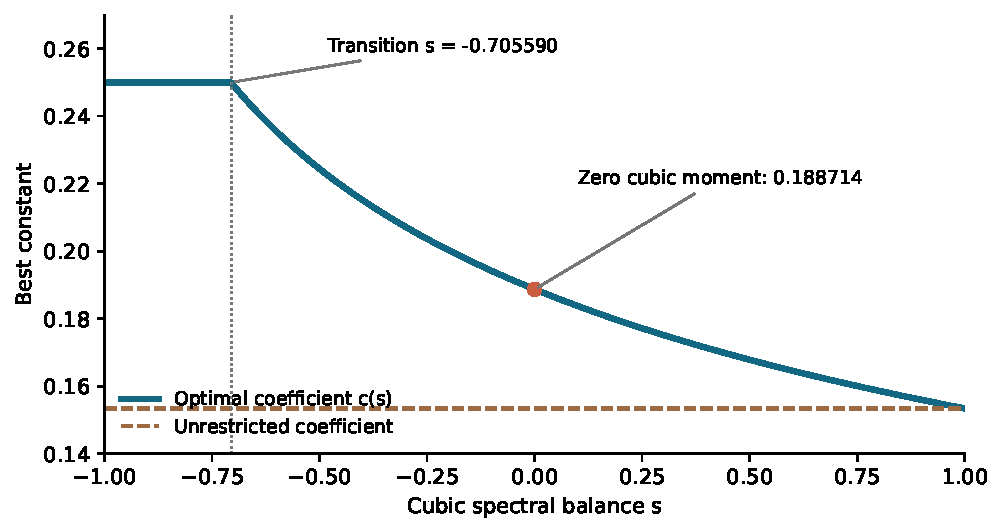
\includegraphics[width=.94\linewidth]{figures/sharp_constant_frontier.pdf}
\caption{The proved optimal coefficient at each cubic spectral balance.
The plateau comes from arbitrarily small normalized deviations; the
decreasing branch comes from normalized deviation $u=1$.}
\label{fig:frontier}
\end{figure}

\subsection{Sharpness for every real parameter}
We supply the exact-parameter argument because rounding positive and
negative multiplicities alone does not prove sharpness when $s$ is irrational.

\begin{lemma}[Exact cubic balance and limiting extremizers]
\label{lem:extremizers}
Fix $s\in(-1,1)$. For all sufficiently large integers $n$, there
are symmetric $n\times n$ matrices $A_n$ with
$\|A_n\|_{\op}=1$, exact cubic ratio $s$, and $v_n/n\to1$ such that
for every fixed $u>0$,
\begin{equation}\label{eq:LDP}
 \lim_{n\to\infty}\frac1{v_n}\log
 \PP\{Q_n\ge v_nu\}=-J_s(u).
\end{equation}
\end{lemma}
\begin{proof}
Put $p_n=\lfloor(1+s)n/2\rfloor$ and $q_n=n-p_n$. For sufficiently
large $n$ both are positive. The function
\[
 F_n(a)=\frac{p_n-q_na^3}{p_n+q_na^2},\qquad 0\le a\le1,
\]
satisfies $F_n(0)=1$, $F_n(1)\le s$, and
\[
 F_n'(a)=-\frac{q_na(2p_n+3p_na+q_na^3)}{(p_n+q_na^2)^2}<0
 \quad(a>0).
\]
There is a unique $a_n\in(0,1]$ with $F_n(a_n)=s$.
Since $F_n(1)=s+O(1/n)$ and the limiting derivative near one is
nonzero, $a_n=1+O_s(1/n)$. Define
\[
 A_n=\diag(1^{[p_n]},(-a_n)^{[q_n]}).
\]
Then $v_n=p_n+q_na_n^2$, $v_n/n\to1$, and the cubic ratio is
exactly $s$. The normalized log-MGFs $K_{A_n}(\theta)/v_n$, together
with their first two derivatives, converge locally uniformly for
$0\le\theta<1/2$ to $H_s(2\theta)$.

The upper bound in \eqref{eq:LDP} follows directly from
Theorem~\ref{thm:signed}. For a lower bound fix $\delta>0$ and tilt
the original probability measure at
$\theta=z_s(u+\delta)/2$:
\[
 \frac{\dd\PP_\theta}{\dd\PP}
 =\exp\{\theta Q_n-K_{A_n}(\theta)\}.
\]
Under this measure,
$\E_\theta Q_n/v_n\to u+\delta$ and
$\Var_\theta(Q_n)/v_n^2=O(1/v_n)$. Chebyshev's inequality therefore
shows that the tilted probability of
\[
 v_n(u+\delta/2)\le Q_n\le v_n(u+3\delta/2)
\]
tends to one. Returning to the original measure gives
\[
 \liminf_n\frac1{v_n}\log\PP(Q_n\ge v_nu)
 \ge -J_s(u+\delta)-\frac\delta2\,\frac{z_s(u+\delta)}2.
\]
Let $\delta\downarrow0$ to obtain \eqref{eq:LDP}.
\end{proof}

\begin{proof}[Completion of Theorem~\ref{thm:frontier}]
If $c(s)=J_s(1)<1/4$, use Lemma~\ref{lem:extremizers} at $u=1$.
If $c(s)=1/4$, first choose a small fixed $u>0$ so that
$J_s(u)/u^2$ is arbitrarily close to $1/4$, then let $n$ grow.
In both cases any larger coefficient contradicts \eqref{eq:LDP}.
For $s=1$ and $s=-1$, use $A_n=I_n$ and $A_n=-I_n$ respectively;
the same tilting argument works, with $u<1$ for the negative case.
Finally $c(s)$ is nonincreasing, so it is valid for the class with
cubic ratio at most $s$. The exact-$s$ subclass already proves optimality.
\end{proof}

For a two-sided bound in the same simple form one obtains
\begin{equation}
 \PP(|Q|\ge t)\le
 2\exp[-c(|s|)\min\{t^2/v,t/L\}].
\end{equation}
The asymmetric sum \eqref{eq:two-sided} usually retains more information.

\section{An explicit four-moment refinement}\label{sec:radau}

For feasible $(s,k)$ with $s<1$, define
\begin{equation}\label{eq:radau-nodes}
 a=\frac{s-k}{1-s},\qquad
 w=\frac{k-s^2}{1-2s+k}.
\end{equation}
Here $-1\le a\le s<1$, $0\le w<1$, and
\begin{equation}\label{eq:nuR}
 \nu_{\mathrm R}=(1-w)\delta_a+w\delta_1
\end{equation}
has moments $1,s,k$. Let
\begin{equation}\label{eq:BR}
 \bRad(s,k;z)=(1-w)g_z(a)+wg_z(1).
\end{equation}
When $s=1$, feasibility forces $k=1$ and we define $a=1,w=1$ and
$\bRad(1,1;z)=g_z(1)$.

\begin{theorem}[Four-moment extremal log-MGF]\label{thm:radau}
For $0\le z<1$,
\begin{equation}\label{eq:hierarchy}
 \frac1rK_A\left(\frac z{2L}\right)
 \le\bRad(s,k;z)\le H_s(z)\le H_1(z).
\end{equation}
For every $0<z<1$, $\bRad(s,k;z)$ is the exact maximum of
$\int g_z\dd\eta$ among all probability measures $\eta$ on $[-1,1]$
with first two moments $s,k$. The same extremizing measure works for
all such $z$. For $0<z<1$, equality in the first inequality holds precisely when every
nonzero eigenvalue of $A$ belongs to $\{aL,L\}$.
\end{theorem}
\begin{proof}
For $s<1$, the inequalities $s^2\le k\le1$ imply $a\le s$ and
$a\ge-1$. Direct substitution verifies the first two moments of
\eqref{eq:nuR}. Let $P_z$ be the quadratic Hermite interpolant to
$g_z$ that matches its value and first derivative at $a$ and its
value at $1$. Explicitly,
\[
 P_z(x)=g_z(a)+g_z'(a)(x-a)
 +\frac{g_z(1)-g_z(a)-g_z'(a)(1-a)}{(1-a)^2}(x-a)^2.
\]
The interpolation remainder is
\[
 g_z(x)-P_z(x)=\frac{g_z'''(\xi_x)}6(x-a)^2(x-1)\le0.
\]
It is strictly negative away from the interpolation nodes. Since
$P_z$ has degree two, integrating it against any admissible measure
gives the same value as integrating against $\nu_{\mathrm R}$.
At that measure interpolation is exact. This proves extremality and
the equality statement. The endpoint secant gives
$\bRad\le H_s$, and the last comparison was proved above. The case
$s=1$ is immediate.
\end{proof}

This proof is the elementary two-node Gauss--Radau argument, applied
to the variance-weighted spectral measure; classical general versions
are described in~\cite{BaiGolub}. For $s^2<k<1$, the improvement
$\bRad(s,k;z)<H_s(z)$ is strict for every $0<z<1$.

\subsection{Closed-form optimization}
If $s<1$ and $k>s^2$, then $w>0$, so the upper endpoint creates a
singularity at $z=1$. Define
\begin{equation}\label{eq:zR}
 z_{\mathrm R}(s,k;u)=
 \frac{2u}{1+u(1+a)+
 \sqrt{[1+u(2s-1-a)]^2+4u^2(k-s^2)}}.
\end{equation}
Set
\begin{equation}\label{eq:JR}
 \jRad(s,k;u)=\frac{u z_{\mathrm R}}2-
                 \bRad(s,k;z_{\mathrm R}).
\end{equation}

\begin{corollary}[Explicit four-moment tail bound]\label{cor:Rtail}
For nondegenerate data as above,
\begin{equation}\label{eq:radau-tail}
 \boxed{\displaystyle\PP(Q\ge t)\le
 \exp[-r\jRad(s,k;tL/v)].}
\end{equation}
The exponent satisfies $\jRad(s,k;u)\ge J_s(u)\ge J_1(u)$.
Computing it from the four scalar inputs requires a square root and
at most two logarithms, with no scalar root search.
\end{corollary}
\begin{proof}
Differentiate \eqref{eq:kernel} with respect to $z$:
\[
 \partial_z g_z(x)=\frac z{2(1-zx)},\qquad
 \partial_z^2g_z(x)=\frac1{2(1-zx)^2}.
\]
The optimizer is unique and satisfies
\begin{equation}\label{eq:Radau-saddle}
 u=z\left(\frac{1-w}{1-za}+\frac w{1-z}\right).
\end{equation}
Clearing denominators produces the quadratic
\[
 [ua+1+a-s]z^2-[1+u(1+a)]z+u=0.
\]
Its unique root in $(0,1)$, written to avoid subtracting nearby quantities,
is \eqref{eq:zR}. Applying Chernoff proves the result. The ordering
of exponents follows from the pointwise ordering of log-MGFs.
\end{proof}

\paragraph{Degenerate data.}
If $k=s^2$, then $w=0$ and the spectral measure is $\delta_s$.
The artificial endpoint $1$ carries no mass and must not restrict
the optimization domain. For $s\ne0$ the rate is
\begin{equation}\label{eq:single}
 \jRad(s,s^2;u)=\frac{us-\log(1+us)}{2s^2},
 \qquad 1+us>0.
\end{equation}
For $s<0$ it is $+\infty$ at $u\ge-1/s$. At $s=0,k=0$ the
relaxed envelope is Gaussian and its rate is $u^2/4$. This last
pair cannot arise from a nonzero finite matrix with $L=\|A\|_{\op}$.
More generally, with that exact norm the boundary $k=s^2$ is attainable
only at $s=1$ or $s=-1$: a one-point nonzero spectral support must
itself attain the norm. All other boundary formulas describe the
relaxed moment problem or a larger supplied norm bound. The endpoint $s=1,k=1$
recovers $J_1$.

\subsection{What moment optimality means}
The extremal assertion in Theorem~\ref{thm:radau} is exact for a
\emph{probability-measure moment problem}. An atom of mass $\omega$
at a nonzero normalized eigenvalue $x$ would require multiplicity
$r\omega/x^2$ in a finite matrix. This need not be an integer.
An atom at zero with positive variance weight is impossible for a
finite spectrum, though it can be approached by many small eigenvalues.
Therefore moment extremality alone does not prove finite-matrix
minimax optimality at every prescribed triple $(r,s,k)$.

Each atom nevertheless has a precise probabilistic realization:
\[
 x\bigl(\chi^2_{r\omega/x^2}-r\omega/x^2\bigr),\qquad x\ne0,
\]
with Gamma-defined, possibly nonintegral degrees of freedom. A zero
atom contributes an independent Gaussian of variance $2r\omega$.
The Radau log-MGF is the sum of these centered log-MGFs after scaling
by $L$. When multiplicities are integral and nodes nonzero, it is
an actual Gaussian quadratic form. For $L$ also to be its exact operator
norm, some positive spectral mass must have $|x|=1$.
Section~\ref{sec:exact} gives such an example with an exact tail calculation.

\subsection{A coefficient for the four-moment envelope}
There is also a simple quadratic/linear coefficient:
\begin{equation}\label{eq:CR}
 \cRad(s,k)=\min\{1/4,\jRad(s,k;1)\}\ge c(s).
\end{equation}
It is valid in \eqref{eq:main} in place of $c(s)$ and is the optimal
coefficient extracted from this log-MGF envelope. This last wording
is distinct from the finite-matrix minimax question just discussed.

\begin{lemma}[An endpoint rule for these rate functions]\label{lem:endpoint}
Let $F(0)=F'(0)=0$, $F''(0)=1/2$, $F''>0$, and $F''''\ge0$ on
its nonnegative log-MGF domain. Suppose $2F'$ covers all positive
values and let $J(u)=\sup_z\{uz/2-F(z)\}$. Then
\[
 \inf_{u>0}\frac{J(u)}{\min\{u^2,u\}}=
 \min\{1/4,J(1)\}.
\]
\end{lemma}
\begin{proof}
Convexity again handles $u\ge1$. In the interior,
$J'''(u)=-F'''(z)/(8F''(z)^3)$. Since $F'''$ is nondecreasing,
$J'''$ can change sign only from positive to negative. For
$G(u)=uJ'(u)-2J(u)$ we have $G(0)=G'(0)=0$ and
$G''(u)=uJ'''(u)$. It follows successively that $G'$ and $G$ either
have one sign throughout or change sign only from positive to negative.
Thus $J(u)/u^2$, whose derivative has sign $G$, cannot take an interior
value below both endpoint values. Its limiting value at zero is $1/4$.
\end{proof}
For $F=\bRad$ the assumptions hold when $w>0$, because
\[
 F''''(z)=3\left[\frac{(1-w)a^2}{(1-za)^4}
                    +\frac{w}{(1-z)^4}\right]\ge0.
\]
The single-node boundary cases follow directly from \eqref{eq:single}.
This proves \eqref{eq:CR}.

\section{Explicit deficits and controlled remainders}\label{sec:remainder}

\subsection{A simple fourth-moment correction to the cubic bound}
The Radau formula is inexpensive, but an additive correction reveals
how the fourth moment improves a cubic-only estimate. Define
\begin{align}
 D(z)&=\frac12\int_0^z\frac{y^3}{(1-y)(1+y)^2}\dd y\label{eq:defect-int}\\
 &=-\frac z2-\frac18\log(1-z)+\frac58\log(1+z)
                  +\frac1{4(1+z)}-\frac14.\label{eq:defect}
\end{align}
It is positive for $0<z<1$ and $D(z)=z^4/8+O(z^5)$.

\begin{proposition}[Spectral spread gives a quantitative gain]
\label{prop:defect}
For $0\le z<1$,
\begin{equation}\label{eq:quant-defect}
 \frac1r K_A\left(\frac z{2L}\right)
 \le H_s(z)-(1-k)D(z).
\end{equation}
For $s>-1$, this implies the explicit bound
\begin{equation}\label{eq:rate-defect}
 \PP(Q\ge t)\le
 \exp\{-r[J_s(u)+(1-k)D(z_s(u))]\}.
\end{equation}
The Radau envelope is at least as strong as the right side of
\eqref{eq:quant-defect} at every $z$.
\end{proposition}
\begin{proof}
For $0\le h<1$, the endpoint secant of $(1-hx)^{-1}$ satisfies
the exact identity
\[
 \frac{1+x}{2(1-h)}+\frac{1-x}{2(1+h)}-\frac1{1-hx}
 =\frac{h^2(1-x^2)}{(1-h^2)(1-hx)}.
\]
Integrating this with $h=za$ against $z^2a\dd a/2$ gives the
secant defect of $g_z$. Since $1-zax\le1+za$, this defect is at least
$(1-x^2)D(z)$. Integration against $\nu$ proves
\eqref{eq:quant-defect}. Evaluation at the old saddle proves
\eqref{eq:rate-defect}. Since \eqref{eq:quant-defect} holds for every
measure with these moments and Radau attains their supremum, it also
bounds $\bRad$.
\end{proof}
The coefficient $D(z)$ is the largest pointwise coefficient in
this secant-defect comparison: the ratio of the defect to $1-x^2$
increases with $x$ and tends to $D(z)$ as $x\downarrow-1$.
Useful elementary bounds are
\begin{equation}
 D(z)\ge\frac{z^4}{8(1+z)},\qquad
 D(z)\ge\frac{27z^4}{256}.
\end{equation}
Indeed $(1-y)(1+y)^2\le1+y\le1+z$, and its maximum on $[0,1]$
is $32/27$.

\subsection{The first information lost by Radau}
Let $a$ be the interior node from \eqref{eq:radau-nodes}, and set
\begin{equation}
 \rho_5=\int(1-x)(x-a)^2\dd\nu(x)\ge0.
\end{equation}
The rational Hermite remainder, followed by
\eqref{eq:kernel-integral}, gives the exact identity
\begin{align}\label{eq:radau-rem}
 \bRad(s,k;z)-\frac1rK_A\left(\frac z{2L}\right)
 &=\frac{z^5}{2}\int\!\int_0^1
 \frac{b^4(1-x)(x-a)^2}
 {(1-zbx)(1-zba)^2(1-zb)}\dd b\dd\nu(x).
\end{align}
Here $b$ is only an integration variable. To verify the identity,
the Hermite interpolant of $(1-hx)^{-1}$ at the double node $a$ and
single node $1$ has excess
\[
 \frac{h^3(1-x)(x-a)^2}{(1-hx)(1-ha)^2(1-h)}.
\]
It agrees at the two nodes and has the required derivative; clearing
denominators verifies the formula directly. Integrating it proves
\eqref{eq:radau-rem}.

Consequently Radau preserves the exact cumulants through fourth order,
and
\begin{equation}
 \bRad-\frac{K_A}{r}=\frac{\rho_5z^5}{10}+O(z^6).
\end{equation}
Uniformly for $0\le z<1$,
\begin{equation}
 \frac{\rho_5z^5}{10(1+z)^4}
 \le\bRad-\frac{K_A}{r}
 \le\frac{\rho_5z^5}{10(1-z)^4}.
\end{equation}
In unnormalized notation, if $p_j=\tr A^j$ and $c=aL$, the leading
physical residual is
\begin{equation}
 R_5=Lp_4-p_5-c^2(Lp_2-p_3)
 =\sum_i\lambda_i^2(L-\lambda_i)(\lambda_i-c)^2\ge0,
\end{equation}
and the log-MGF difference is $(16/5)R_5\theta^5+O(\theta^6)$.
These expressions identify exactly what a fifth spectral moment could
improve. Their nonnegativity remains valid for indefinite matrices.

\section{An exact harmonic example with rational tail certificates}
\label{sec:exact}

Consider a matrix with $m$ eigenvalues $1$ and $8m$ eigenvalues $-1/2$:
\begin{equation}\label{eq:example}
 A=\diag(1^{[m]},(-1/2)^{[8m]}).
\end{equation}
Its parameters are
\[
 L=1,\quad v=r=3m,\quad s=0,\quad k=\frac12,
 \qquad\nu=\frac13\delta_1+\frac23\delta_{-1/2}.
\]
This is exactly the Radau measure for these moments. At normalized
deviation $u=1$, the optimizer is $z_{\mathrm R}=2/3$ and
\begin{equation}\label{eq:Jexample}
 J_*:=\jRad(0,1/2;1)
 =\frac43\log\frac43-\frac16\log3
 =0.200474048491\ldots.
\end{equation}
The comparison is therefore exact at the log-MGF level:
\begin{center}
\begin{tabular}{@{}lc@{}}
\toprule
Information used & Exponent divided by $v$, at $t=v$\\
\midrule
Norm and variance & $0.153426409720\ldots$\\
Also the signed cubic moment & $0.188714038110\ldots$\\
Also the fourth moment & $0.200474048491\ldots$\\
Full spectrum & $0.200474048491\ldots$\\
\bottomrule
\end{tabular}
\end{center}
The fourth moment gains another $6.23\%$ in this exponent beyond the
cubic-moment bound.

\subsection{An exact probability, without simulation}
For this subsection only, put $m=2\ell$ with positive integer $\ell$.
Then $v=6\ell$, and
\[
 Q\overset d=X-\frac12Y+6\ell,
 \qquad X\sim\chi^2_{2\ell},\quad Y\sim\chi^2_{16\ell}
\]
with independent $X,Y$. At $Q\ge v$, the event is $X\ge Y/2$.
The change of variables $B=X/(X+Y)$ in the joint Gamma density shows
that $B$ has beta density proportional to $b^{\ell-1}(1-b)^{8\ell-1}$.
For positive integer beta parameters, differentiation of the binomial
tail and checking its endpoint value gives
\begin{equation}\label{eq:rational}
 P_\ell:=\PP(Q\ge v)
 =3^{-(9\ell-1)}\sum_{j=0}^{\ell-1}
       \binom{9\ell-1}{j}2^{9\ell-1-j}.
\end{equation}
Thus every value is an exact rational number; $P_1=256/6561$.
The code stores the integer numerator and denominator, not a Monte
Carlo estimate.

\begin{proposition}[Sharp equivalent and first correction]
\label{prop:asymptotic}
For the probabilities in \eqref{eq:rational},
\begin{equation}\label{eq:tail-asymptotic}
 P_\ell=
 \frac{e^{-6\ell J_*}}{3\sqrt{\pi\ell}}
 \left(1-\frac{505}{864\ell}+O(\ell^{-2})\right).
\end{equation}
In particular $-\log P_\ell/(6\ell)\to J_*$, so the four-moment
exponent is asymptotically attained by actual finite matrices.
\end{proposition}
\begin{proof}
Let $T_\ell$ be the last summand of \eqref{eq:rational}, including the
common normalization. A binomial identity gives
\[
 T_\ell=\frac13\binom{9\ell}{\ell}
                  \frac{2^{8\ell}}{3^{9\ell}}.
\]
Stirling's formula with its usual controlled remainder~\cite{DLMF}
yields
\begin{equation}\label{eq:lastterm}
 T_\ell=\frac{e^{-6\ell J_*}}{4\sqrt{\pi\ell}}
       \left(1-\frac{73}{864\ell}+O(\ell^{-2})\right).
\end{equation}
Moving backward by $h$ summands multiplies $T_\ell$ by
\[
 R_{\ell,h}=\prod_{i=1}^{h}\frac{2(\ell-i)}{8\ell+i},
 \qquad0\le h\le\ell-1.
\]
Each factor is at most $1/4$, and for fixed $h$,
$R_{\ell,h}\to4^{-h}$. This already proves the leading equivalent
by dominated convergence, since $\sum_{h\ge0}4^{-h}=4/3$.

For the correction, expand the logarithm of the product:
\[
 R_{\ell,h}=4^{-h}
 \left(1-\frac{9h(h+1)}{16\ell}
 +O\left(\frac{(1+h)^4}{\ell^2}\right)\right),
 \qquad h\le\ell^{1/8}.
\]
The remainder is uniform on this range by the Taylor remainder for
$\log(1+x)$. The sum beyond this range is bounded by a geometric
tail, hence smaller than any inverse power of $\ell$. Since
\[
 \frac{\sum_{h\ge0}h(h+1)4^{-h}}{\sum_{h\ge0}4^{-h}}=\frac89,
\]
we obtain
$\sum_hR_{\ell,h}=(4/3)(1-1/(2\ell)+O(\ell^{-2}))$.
Multiplication by \eqref{eq:lastterm} proves
\eqref{eq:tail-asymptotic}.
\end{proof}

There is also an exact finite sandwich:
\begin{equation}\label{eq:finite-sandwich}
 T_\ell\le P_\ell\le
 \frac{T_\ell}{1-2(\ell-1)/(8\ell+1)}.
\end{equation}
It follows because each successive backward ratio is at most the
first. The included standard-library script verifies this sandwich in
exact rational arithmetic.

\begin{figure}[htbp]
\centering
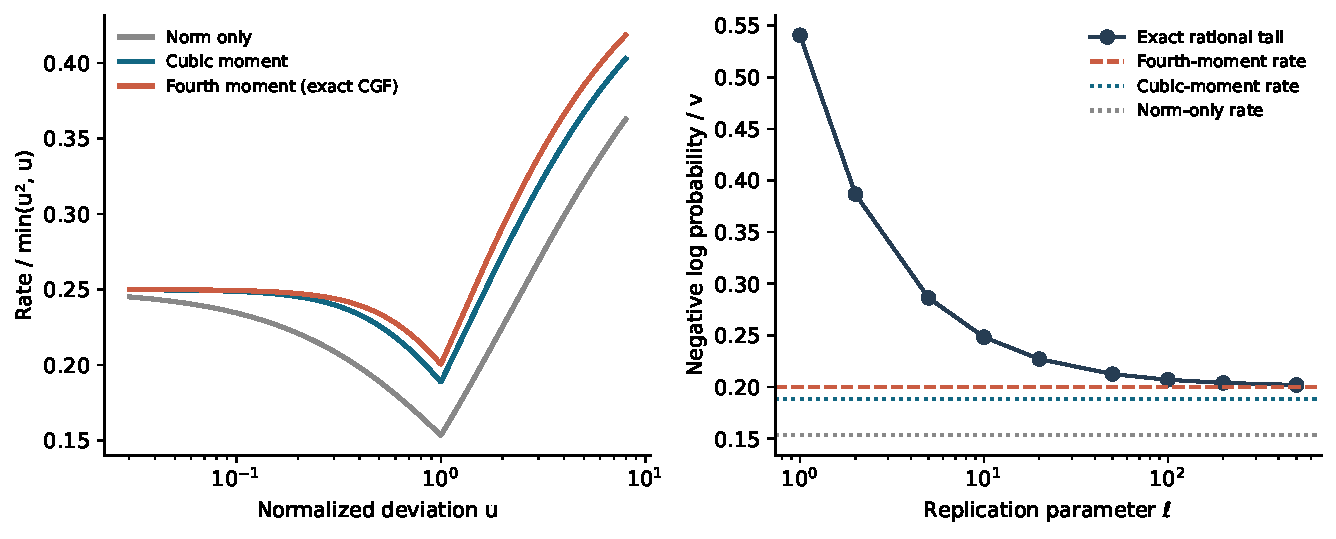
\includegraphics[width=\linewidth]{figures/rate_and_exact_tail.pdf}
\caption{The example \eqref{eq:example}. Left: normalized exponents
from two, three, and four moments. Right: exact rational tails approach
the fourth-moment exponent. The horizontal variable $\ell$ is the
integer replication parameter of this section.}
\label{fig:exact}
\end{figure}

\begin{center}
\small
\begin{tabular}{@{}rrrr@{}}
\toprule
$\ell$ & Dimension & $-\log P_\ell/(6\ell)$ &
$3\sqrt{\pi\ell}\,e^{6\ell J_*}P_\ell$\\
\midrule
1 &18&0.5406201441&0.6908038618\\
5 &90&0.2863652587&0.9038967705\\
20&360&0.2271143501&0.9723953442\\
100&1800&0.2071063054&0.9942249100\\
500&9000&0.2020671979&0.9988338567\\
\bottomrule
\end{tabular}
\end{center}
The first ratio tends to $J_*$ and the second to one. These finite
data check the prediction but do not replace its proof.

\section{Applications}

\subsection{Harmonic Gibbs fluctuations and free energy}
Let $K$ be a real symmetric positive-definite stiffness matrix and
$\beta>0$ the inverse temperature. The Gibbs density for
\[
 \mathcal H(x)=\frac12x^{\mathsf T}Kx
\]
is Gaussian with covariance $\beta^{-1}K^{-1}$. For any symmetric
matrix $B$, define $\mathcal O_B(x)=x^{\mathsf T}Bx/2$. Whitening
gives the exact identity
\begin{equation}\label{eq:harmonic}
 2\beta(\mathcal O_B-\E\mathcal O_B)
 \overset d=g^{\mathsf T}Ag-\tr A,
 \qquad A=K^{-1/2}BK^{-1/2}.
\end{equation}
Every bound above therefore applies at threshold $t=2\beta h$ for
an observable deviation $h$.

The same determinant is a free-energy difference:
\begin{equation}
 \E e^{\theta\mathcal O_B}
 =\left[\frac{\det K}{\det(K-(\theta/\beta)B)}\right]^{1/2}
\end{equation}
whenever the perturbed stiffness matrix is positive definite. The
centering subtracts $\theta\tr A/(2\beta)$ from its logarithm.
Thus signed moment information controls an exact finite-volume
free-energy response, as well as a probability tail.

When $B=K$, total energy is a scaled chi-square variable. More
informatively, let $B$ select the difference of energies in two
orthogonal normal-mode sectors. Then $A$ has eigenvalues $+1$ and
$-1$; equal sector sizes give $s=0$ and attain the signed envelope.
The choice $\mathcal O=\mathcal H_+-\frac12\mathcal H_-$, with
one eighth as many positive-sector modes, gives
\eqref{eq:example}. The cancellation advantage has an immediate
physical meaning: it concerns contrasts between fluctuating mode
energies. These statements require a normalizable harmonic Gibbs
measure; unconstrained zero modes must first be removed or confined.

\subsection{Sharper guarantees for ordinary Gaussian trace estimates}
For independent standard Gaussian probes $g_1,\ldots,g_N$, set
\[
 \widehat\tau_N=\frac1N\sum_{j=1}^N g_j^{\mathsf T}Ag_j.
\]
Its centered error is a quadratic form with matrix
$\diag(A/N,\ldots,A/N)$. The parameters transform as
\[
 L_N=L/N,\quad v_N=v/N,\quad r_N=Nr,\quad s_N=s,\quad k_N=k.
\]
For an absolute tolerance $\varepsilon>0$, put
$u=\varepsilon L/v$. Then
\begin{equation}\label{eq:trace}
 \PP\{\widehat\tau_N-\tr A\ge\varepsilon\}
 \le e^{-Nr\jRad(s,k;u)}.
\end{equation}
Together with reflection, a sufficient sample count for failure
probability at most $\delta$ is
\begin{equation}\label{eq:N}
 N\ge\frac{\log(2/\delta)}{
 r\min\{\jRad(s,k;u),\jRad(-s,k;u)\}}.
\end{equation}
Replacing $\jRad$ by $J$ gives the cubic-only guarantee.

For $s=0$, the simplified coefficient guarantee improves the
unrestricted sufficient sample count by the ratio
$c(1)/c(0)=0.81301005\ldots$ before integer rounding, approximately
$18.70\%$ fewer probes. This comparison holds between the stated
sufficient bounds; it is not an empirical performance claim or an
information-theoretic lower bound for all trace-estimation algorithms.
It also does not change the $\varepsilon^{-2}$ small-error order of
the ordinary Gaussian sample mean. Indefinite trace estimation and
matrix-function applications are studied in~\cite{Cortinovis}; more
sophisticated methods such as Hutch++ address different query
complexity goals~\cite{Hutchpp}.

\subsection{Diagonal-free subgaussian forms}
The Gaussian comparison used by Dadush et al.~\cite{DGO} also transfers
our bounds to a broader class without decoupling losses.

\begin{proposition}\label{prop:subgaussian}
Suppose $X_1,\ldots,X_n$ are independent and
$\E e^{hX_i}\le e^{h^2/2}$ for every real $h$. If $A$ is symmetric
with zero diagonal, then every Chernoff upper-tail bound obtained from
the Gaussian log-MGF envelopes above holds for $X^{\mathsf T}AX$,
with the same matrix parameters.
\end{proposition}
\begin{proof}
Conditional on all coordinates except $i$, the exponent
$\theta X^{\mathsf T}AX$ is affine in $X_i$, because $A_{ii}=0$.
The defining subgaussian MGF inequality permits replacement of that
coordinate by an independent standard Gaussian without decreasing
the conditional exponential expectation. Replace coordinates one
at a time, always retaining the original quadratic integrand.
Tonelli's theorem handles the nonnegative integrand. Thus
\[
 \E e^{\theta X^{\mathsf T}AX}\le
 \E e^{\theta g^{\mathsf T}Ag}.
\]
The diagonal condition also gives $\tr A=0$, so the Gaussian
right side is precisely the MGF of the centered Gaussian form used above.
\end{proof}
For proxy parameter $\sigma$, meaning
$\E e^{hX_i}\le e^{\sigma^2h^2/2}$, replace the threshold by
$t/\sigma^2$. No claim of sharpness for every subgaussian subclass
is needed for this transfer.

\subsection{Triangle-free graphs and random cuts}
Let $G$ be a simple triangle-free graph with $m>0$ edges and
adjacency matrix $A$. Closed-walk counting gives
\begin{equation}
 \tr A^2=2m,\qquad \tr A^3=0,
\end{equation}
so $s=0$. If $X_i$ are independent uniform signs, the cut size is
\[
 \mathrm{Cut}=\frac m2-\frac14X^{\mathsf T}AX.
\]
Applying Proposition~\ref{prop:subgaussian} to either tail gives
\begin{equation}\label{eq:cut}
 \PP\!\left\{\mathrm{Cut}\le\frac m2-d\right\}
 \le\exp\!\left[-c(0)\min\left\{\frac{8d^2}{m},\frac{4d}{L}\right\}\right],
 \qquad d>0,
\end{equation}
and the same bound for $\mathrm{Cut}\ge m/2+d$.
This uses vanishing cubic trace, which is weaker than spectral
symmetry or bipartiteness. A fourth-moment refinement follows from
\begin{equation}
 \tr A^4=2m+4\sum_x\binom{\deg x}{2}+8N_4,
\end{equation}
where $N_4$ counts unoriented simple four-cycles. The terms count
closed walks using one edge, two adjacent edges, or four distinct edges.
For instance the five-cycle has $L=2,v=10,k=3/4$ and Radau nodes
$-3/4,1$ with upper mass $3/7$.

A certified upper bound $L\ge\|A\|_{\op}$ can replace the exact
norm throughout the valid inequalities, after recomputing $r,s,k$.
For graphs one may take the maximum degree. This can loosen the
bound; claims of the optimal coefficient use the actual norm.
Special graph families may admit stronger combinatorial estimates
than \eqref{eq:cut}; no optimal random-cut constant is asserted.

\section{Computation and reproducible verification}\label{sec:verification}

\subsection{What the included implementation computes}
The module \texttt{code/spectral\_concentration.py} computes the
norm-only rate, signed rate and coefficient, Radau nodes, Radau
rate and coefficient, directional and two-sided bounds, and a
sufficient Gaussian-probe count. The input may be spectral moments
or an explicitly supplied eigenvalue list. The formulas themselves
do not require eigendecomposition once the moments are available.

If the complete spectrum is supplied, moment formation costs
$O(n)$ arithmetic operations and each bound evaluation costs $O(1)$.
For a general matrix accessible only by matrix-vector products,
obtaining exact traces $\tr A^3$ and $\tr A^4$ may be costly.
They are not free inputs. In particular, plugging unqualified noisy
moment estimates into an extremal formula does not produce a
certified probability inequality. A rigorous estimated-moment
implementation must first construct a simultaneous confidence set
and maximize over that set, accounting for its failure probability.
That extension is a research problem below.

The numerical implementation uses \texttt{log1p} and convergent
series near zero. At extreme tail sizes a floating-point saddle can
round to a log-MGF singularity; the implementation chooses a
representable point inside the domain. Any such point yields a
valid Chernoff expression in exact arithmetic, although it need not
be the exact optimizer. The implementation uses ordinary floating
point and is not an outward-rounded interval proof.

\subsection{Checks and exact artifacts}
Run
\begin{quote}\ttfamily
python3 code/reproduce.py
\end{quote}
from the package directory. It creates both figures and the CSV/JSON
tables. The fixed seed is \texttt{20261008}; no random samples of
$Q$ and no downloaded dataset are used. The audit includes:
\begin{itemize}
\item Five symbolic identities: the signed saddle derivative, the
coefficient derivative identity, the reciprocal secant remainder,
the defect antiderivative, and the Radau saddle polynomial.
\item A deterministic set of 187 signed spectra, including
projections, negative projections, balanced spectra, two-level
spectra, zero eigenvalues, small eigenvalues, and random signed spectra.
\item 1,309 comparisons of exact, Radau, cubic, and norm log-MGFs,
and 1,122 comparisons of the resulting tail exponents.
\item 45 independent scalar minimizations compared with the
closed-form Radau optimizer, and 20 independent high-precision
integrals for the spectral kernel.
\item Nine exact rational tail certificates from
\eqref{eq:rational}, including a matrix of dimension $9{,}000$.
The standard-library certificate script also verifies
\eqref{eq:finite-sandwich} without rounding.
\end{itemize}
The hierarchy checks agree to floating-point roundoff; the detailed
summary records the tolerances and maximum discrepancies. Boundary
regressions cover invalid data and very large finite deviations.
These computational checks support the derivations but are neither
substitutes for the proofs nor a formal verification claim.

\section{Interpretation, prior-art audit, and limits}\label{sec:scope}

\subsection{What has been strengthened}
The main theorem replaces one universal constant by the exact
optimal function of a measurable spectral parameter. It completely
characterizes the competition between small deviations and the
quadratic/linear regime boundary. Its optimality is proved over
actual finite-dimensional matrices at every exact real parameter,
not only over formal Gamma laws.

The fourth-moment theorem gives a stronger full exponent with a
closed optimizer. Its extremality is with respect to a specified
moment relaxation, its equality cases are explicit, and its
first omitted information has a nonnegative integral remainder.
An actual matrix family attains the refinement and admits exact
finite probability certificates. The gains are relevant to
signed quadratic statistics, harmonic energy contrasts, and
diagonal-free subgaussian forms.

\subsection{What the literature review supports}
The most relevant inspected sources were the original norm-only
Gamma bound of Dadush et al., Gallagher et al.'s trace-based
Gaussian concentration bounds, Moshksar's September 2026 revision,
Pang's September 2026 Gamma comparison, and the classical
Bai--Golub quadrature treatment~\cite{DGO,Gallagher,Moshksar,Pang,BaiGolub}.
Targeted searches used the exact proposed constants and the
phrases signed cubic moment, skewness-dependent concentration,
Gaussian quadratic form, and Gauss--Radau moment envelope.
No matching theorem for the complete $c(s)$ frontier and its
transition was located. Gallagher et al.'s discussion of
asymmetry in the positive and negative spectrum is especially
close in motivation.

An initial candidate was the unconditional coefficient
$(1-\log2)/2$. The older literature ruled out a novelty claim
for that coefficient. This matters because Moshksar's recent
discussion advertises smaller coefficients from particular
inequality families. Those numbers are not a sufficient baseline
for asserting a new global best constant. The comparisons in this
article instead use the stronger established Gamma bound.

\subsection{Limits of the result}
The concentration problem is a central Gaussian problem, with a
specified additional subgaussian extension for zero diagonal.
No general noncentral or arbitrarily dependent subgaussian
extension is proved. No asymptotic improvement in a matrix-query
complexity exponent is claimed. The physics application concerns
normalizable harmonic systems, and does not prove a new theorem
about interacting critical spin models. The word optimal in the
four-moment statement must retain its moment-relaxation qualifier.

Publication would require a broader literature check and external
review of the proofs. These are limits on priority and validation,
not assumptions left inside the mathematical arguments.

\section{Further research questions and a proposed program}

\begin{enumerate}[leftmargin=*]
\item \textbf{Finite-matrix optimality with both moments fixed.}
Determine the exact best coefficient for prescribed
$(r,s,k)$ when spectral multiplicities must be integers. The Radau
envelope is a computable upper log-MGF bound, but its formal
extremizer need not be a matrix. Start with two-node moment data
and quantify the gap caused by multiplicity rounding. This is the
most direct remaining mathematical question.

\item \textbf{A complete two-parameter sharp frontier.}
For the relaxation, \eqref{eq:CR} gives an explicit function on
$s^2\le k\le1$. Describe its level sets, its $1/4$ plateau, and the
boundary where $\jRad(s,k;1)=1/4$. Decide when its sharp
coefficient is realized by actual matrix sequences with both
normalized moments exact.

\item \textbf{Moment uncertainty with rigorous confidence guarantees.}
Develop a robust optimization over simultaneous confidence intervals
for $v,p_3,p_4,L$. The objective is to preserve a substantial part of
the exponent gain while including the cost of estimating moments.
Signed $p_3$ makes naive coordinatewise substitution unsafe. A useful
deliverable would be a globally certified low-dimensional optimizer.

\item \textbf{Higher spectral-moment hierarchy.}
Use right Gauss--Radau rules with more nodes to retain
$p_2,\ldots,p_{2m+2}$. Positivity of all spectral derivatives
suggests a monotone sequence of log-MGF envelopes. Prove usable
nonasymptotic convergence estimates that remain informative as the
saddle approaches its pole; identify which additional moments
provide the greatest improvement per unit computational work.

\item \textbf{Separate positive and negative spectral endpoints.}
If $\lambda_{\max}$ and $-\lambda_{\min}$ differ markedly, the
symmetric interval $[-L,L]$ is wasteful. The Hermite proof already
works on a general interval. Determine the optimal coefficient
surface after a normalization that treats the variance and both
endpoints naturally, including all boundary regimes.

\item \textbf{Noncentral Gaussian quadratic forms.}
The noncentral log-MGF has an additional rational spectral term
depending on the mean vector. It is natural to introduce both
variance-weighted and mean-weighted measures. The difficult part
is a joint moment constraint, rather than applying two independent
upper bounds that lose alignment information.

\item \textbf{Sharper prefactors for moment classes.}
The present bounds optimize exponential rates. The exact example
has a factor proportional to $r^{-1/2}$. Investigate uniform
prefactor improvements under conditions controlling the tilted
variance and the number of effective spectral modes. Such results
would be substantially stronger for small failure probabilities.

\item \textbf{Graph structure beyond triangle counts.}
For random cuts, $p_3$ and $p_4$ are short closed-walk counts.
Combine the spectral envelope with combinatorial restrictions on
these counts, and compare against specialized cut bounds. The
zero-diagonal Gaussian comparison need not be sharp for random
signs; identifying the additional slack could lead to a larger
graph-specific constant.

\item \textbf{Certified numerical implementation.}
Implement outward-rounded logarithms, square roots, and moment
feasibility checks. Construct confidence bounds that remain valid
under finite precision, and formalize the scalar interpolation and
coefficient lemmas in Lean. The proof's division into spectral
integration, elementary calculus, and exponential tilting makes
these independent verification targets.

\item \textbf{Weakly anharmonic systems.}
For a Gibbs measure close to a harmonic reference, quantify the
change of measure needed to transfer a signed-moment tail bound.
Any such theorem must account explicitly for the interaction
remainder and its temperature and volume dependence. The harmonic
result supplies a reference inequality; it is not itself a
justification for an interacting-model limit.
\end{enumerate}

\appendix
\section{A finite-rank certificate for the established endpoint constant}
\label{app:gamma}
The unrestricted coefficient can be checked without invoking an
asymptotic theorem as a black box. Let $Y\sim\chi^2_d$, $d\ge1$,
and $\varepsilon>0$. Write $h(\varepsilon)=\varepsilon-\log(1+\varepsilon)$.
Then
\begin{equation}\label{eq:gamma-sandwich}
 \frac{e^{-dh(\varepsilon)/2}}{\varepsilon\sqrt{\pi d}}
 \frac{e^{-1/(6d)}}{1+2(1+\varepsilon)/(d\varepsilon^2)}
 \le\PP\{Y\ge d(1+\varepsilon)\}
 \le\frac{e^{-dh(\varepsilon)/2}}{\varepsilon\sqrt{\pi d}}.
\end{equation}
These are elementary consequences of the Gamma integral and standard
Stirling bounds~\cite{DLMF}; they are included as a reproducible
sharpness certificate, not as a new incomplete-Gamma estimate.

For completeness let $a=d/2$, $c=1+\varepsilon$, and
$f(x)=x-1-\log x$. Substitution in the Gamma tail gives the
integral $I=\int_c^\infty e^{-af(x)}\dd x/x$, multiplied by
$a^ae^{-a}/\Gamma(a)$. Integration by parts yields
\[
 I=\frac{e^{-af(c)}}{a\varepsilon}
 -\frac1a\int_c^\infty\frac{x}{(x-1)^2}
                         e^{-af(x)}\frac{\dd x}{x}.
\]
The bracket is decreasing on $(1,\infty)$. If
$M=e^{-af(c)}/(a\varepsilon)$, it follows that
$M/[1+c/(a\varepsilon^2)]\le I\le M$.
The scaled Gamma function satisfies
$1<\Gamma^*(a)<e^{1/(12a)}$, which proves
\eqref{eq:gamma-sandwich}. At $\varepsilon=1$ this becomes
$e^{-d\cstar}/\sqrt{\pi d}$ times a factor tending to one.
Any coefficient greater than $\cstar$ must therefore fail in a
sufficiently large finite dimension.

\section{Package contents and reproduction}
The package contains the manuscript source and PDF, the principal
Python module, a reproduction script, a standard-library exact
certificate script, generated CSV and JSON data, vector and raster
figures, build instructions, and a source/provenance record. The
PDF is generated from this source with \texttt{pdflatex}. There
are no external figure downloads and no runtime network requirement.

The exact-rational certificate script can run without scientific
Python libraries. Reproducing figures and all audits requires
NumPy, SciPy, Matplotlib, SymPy, and mpmath. Tested versions are
recorded in the verification JSON. The user may integrate the
source, results, and code into a research repository; no external
repository was modified in preparing this package.

\begin{thebibliography}{99}
\raggedright
\bibitem{openai} OpenAI, \emph{Mathematical manuscripts and supporting
proof artifacts}, public repository, inspected 8 October 2026.
\url{https://github.com/openai/math}.

\bibitem{bloch} OpenAI mathematical manuscript collection,
\emph{The first lattice correction to Bloch's law}, 5 October 2026,
family 271. Repository path
\url{preprints/The-first-lattice-correction-to-Blochs-law-October-5-2026/}.
The section on the explicit lattice correction was used for
methodological inspiration, not as a theorem dependency.

\bibitem{LM} B. Laurent and P. Massart,
\emph{Adaptive estimation of a quadratic functional by model selection},
Annals of Statistics \textbf{28} (2000), 1302--1338.
\url{https://doi.org/10.1214/aos/1015957395}.

\bibitem{DGO} D. Dadush, C. Guzm\'an, and N. Olver,
\emph{Fast, deterministic and sparse dimensionality reduction},
Proceedings of SODA 2018, 1330--1344.
\url{https://doi.org/10.1137/1.9781611975031.87}.
Author-hosted copy: \url{https://ir.cwi.nl/pub/27624/27624.pdf}.

\bibitem{Gallagher} R. E. Gallagher, L. J. M. Aslett, D. Steinsaltz,
and R. R. Christ, \emph{Improved concentration bounds for Gaussian
quadratic forms}, arXiv:1911.05720.
\url{https://arxiv.org/abs/1911.05720}.

\bibitem{Moshksar} K. Moshksar, \emph{Refining concentration bounds for
Gaussian quadratic chaos with applications}, arXiv:2412.03774v5,
13 September 2026. \url{https://arxiv.org/html/2412.03774v5}.

\bibitem{Pang} Z. Pang, \emph{A Gamma envelope and sharp moment
inequalities for Gaussian quadratic forms}, arXiv:2609.05914v1,
5 September 2026. \url{https://arxiv.org/abs/2609.05914}.

\bibitem{BaiGolub} Z. Bai and G. Golub, \emph{Computation of large-scale
quadratic forms and transfer functions using the theory of moments,
quadrature and Pad\'e approximation}, in \emph{Modern Methods in
Scientific Computing and Applications}, 2002.
Author-hosted manuscript: \url{https://web.cs.ucdavis.edu/~bai/publications/baigolub02.pdf}.

\bibitem{Cortinovis} A. Cortinovis and D. Kressner,
\emph{On randomized trace estimates for indefinite matrices with an
application to determinants}, Foundations of Computational Mathematics,
published online 2021. \url{https://doi.org/10.1007/s10208-021-09525-9}.

\bibitem{Hutchpp} R. A. Meyer, C. Musco, C. Musco, and D. P. Woodruff,
\emph{Hutch++: Optimal stochastic trace estimation}, SOSA 2021.
\url{https://pmc.ncbi.nlm.nih.gov/articles/PMC8553228/}.

\bibitem{DLMF} F. W. J. Olver et al. (eds.),
\emph{NIST Digital Library of Mathematical Functions}, Sections 5.11
and 8.11, Gamma and incomplete-Gamma asymptotics and remainder bounds.
\url{https://dlmf.nist.gov/5.11}; \url{https://dlmf.nist.gov/8.11}.
\end{thebibliography}
\end{document}
